\section{Winoground}

\subsection{Capabilities of Encoders}

\subsubsection{Baseline}

See \cref{tab:perplexity-and-length-correlations-baseline}

\begin{table}[ht]
\centering
\begin{adjustbox}{max width=\textwidth}
\begin{tabular}{l|rr|rrrrrr}
\toprule
 & \multicolumn{2}{c|}{Perplexity} &  \multicolumn{6}{c}{Caption Length}\\
 & \multicolumn{2}{c|}{Text-Image} &  \multicolumn{2}{c}{Text} &  \multicolumn{2}{c}{Image} &  \multicolumn{2}{c}{Group}\\
 Model      &   Corr. &   p-value & Corr. &   p-value & Corr. &   p-value & Corr. &   p-value\\\midrule 
  MTurk Human                  & 0.05           & 0.07          & \textbf{0.11}  & \textbf{0.03} & \textbf{0.20}  & \textbf{0.00} & \textbf{0.20}  & \textbf{0.00} \\
 VinVL                        & \textbf{-0.05} & \textbf{0.04} & \textbf{-0.11} & \textbf{0.03} & \textbf{-0.18} & \textbf{0.00} & \textbf{-0.20} & \textbf{0.00} \\
 UNITER$_{large}$             & -0.01          & 0.57          & -0.08          & 0.13          & -0.06          & 0.20          & \textbf{-0.16} & \textbf{0.00} \\
 UNITER$_{base}$              & -0.03          & 0.22          & \textbf{-0.15} & \textbf{0.00} & \textbf{-0.11} & \textbf{0.03} & \textbf{-0.14} & \textbf{0.00} \\
 ViLLA$_{large}$              & -0.02          & 0.39          & -0.05          & 0.32          & \textbf{-0.13} & \textbf{0.01} & \textbf{-0.12} & \textbf{0.01} \\
 ViLLA$_{base}$               & -0.04          & 0.13          & \textbf{-0.14} & \textbf{0.01} & \textbf{-0.12} & \textbf{0.01} & \textbf{-0.11} & \textbf{0.03} \\
 VisualBERT$_{base}$          & -0.04          & 0.15          & -0.09          & 0.07          & -0.07          & 0.14          & -0.06          & 0.22          \\
 ViLT (ViT-B/32)              & -0.04          & 0.16          & -0.09          & 0.06          & \textbf{-0.20} & \textbf{0.00} & \textbf{-0.16} & \textbf{0.00} \\
 LXMERT                       & -0.04          & 0.12          & -0.00          & 0.97          & -0.05          & 0.32          & \textbf{-0.11} & \textbf{0.02} \\
 ViLBERT$_{base}$             & -0.04          & 0.11          & -0.09          & 0.09          & \textbf{-0.15} & \textbf{0.00} & \textbf{-0.14} & \textbf{0.00} \\
 UniT$_{ITM Finetuned}$       & -0.01          & 0.73          & -0.03          & 0.53          & -0.05          & 0.32          & -0.02          & 0.73          \\
 FLAVA$_{ITM}$                & -0.03          & 0.22          & \textbf{-0.21} & \textbf{0.00} & \textbf{-0.22} & \textbf{0.00} & \textbf{-0.23} & \textbf{0.00} \\
 FLAVA$_{Contrastive}$        & \textbf{-0.06} & \textbf{0.01} & \textbf{-0.15} & \textbf{0.00} & \textbf{-0.25} & \textbf{0.00} & \textbf{-0.19} & \textbf{0.00} \\
 CLIP (ViT-B/32)              & -0.04          & 0.09          & \textbf{-0.27} & \textbf{0.00} & \textbf{-0.19} & \textbf{0.00} & \textbf{-0.22} & \textbf{0.00} \\
 VSE++$_{COCO}$ (ResNet)      & \textbf{-0.05} & \textbf{0.04} & -0.03          & 0.60          & -0.02          & 0.74          & 0.01           & 0.90          \\
 VSE++$_{COCO}$ (VGG)         & -0.04          & 0.08          & -0.02          & 0.65          & 0.03           & 0.50          & 0.03           & 0.56          \\
 VSE++$_{Flickr30k}$ (ResNet) & -0.02          & 0.43          & -0.01          & 0.80          & 0.01           & 0.91          & 0.02           & 0.67          \\
 VSE++$_{Flickr30k}$ (VGG)    & 0.01           & 0.74          & -0.09          & 0.07          & -0.07          & 0.18          & \textbf{-0.10} & \textbf{0.04} \\
 VSRN$_{COCO}$                & \textbf{-0.07} & \textbf{0.01} & -0.03          & 0.60          & -0.05          & 0.30          & -0.05          & 0.36          \\
 VSRN$_{Flickr30k}$           & -0.02          & 0.32          & -0.03          & 0.60          & -0.10          & 0.06          & -0.05          & 0.29          \\
\bottomrule
\end{tabular}
\end{adjustbox}
\caption{(left) The correlation between model image-caption scores and the caption perplexity from GPT2. (right) The correlation between the model text, image and group scores and the caption length.}
\label{tab:perplexity-and-length-correlations-baseline}
\end{table}

\subsubsection{Ours}

See \cref{tab:perplexity-and-length-correlations-ours}

\begin{table}[ht]
\centering
\begin{adjustbox}{max width=\textwidth}
\begin{tabular}{l|rr|rrrrrr}
\toprule
 & \multicolumn{2}{c|}{Perplexity} &  \multicolumn{6}{c}{Caption Length}\\
 & \multicolumn{2}{c|}{Image-Caption} &  \multicolumn{2}{c}{Text} &  \multicolumn{2}{c}{Image} &  \multicolumn{2}{c}{Group}\\
 Model      &   Corr. &   p-value & Corr. &   p-value & Corr. &   p-value & Corr. &   p-value\\\midrule 
MTurk Human                         & 0.05           & 0.07          & \textbf{0.11}  & \textbf{0.03} & \textbf{0.20}  & \textbf{0.00} & \textbf{0.20}  & \textbf{0.00} \\
 ViLT (ViT-B/32)                     & -0.04          & 0.08          & \textbf{-0.12} & \textbf{0.02} & -0.07          & 0.17          & -0.05          & 0.35          \\
 ViLT$_{COCO}$ (ViT-B/32)            & -0.05          & 0.06          & \textbf{-0.21} & \textbf{0.00} & \textbf{-0.16} & \textbf{0.00} & \textbf{-0.17} & \textbf{0.00} \\
 ViLT$_{Flickr30k}$ (ViT-B/32)       & \textbf{-0.05} & \textbf{0.03} & \textbf{-0.11} & \textbf{0.03} & \textbf{-0.17} & \textbf{0.00} & \textbf{-0.14} & \textbf{0.01} \\
 FLAVA$_{ITM}$                       & -0.03          & 0.22          & \textbf{-0.21} & \textbf{0.00} & \textbf{-0.22} & \textbf{0.00} & \textbf{-0.23} & \textbf{0.00} \\
 FLAVA$_{ITC}$                       & \textbf{-0.06} & \textbf{0.01} & \textbf{-0.15} & \textbf{0.00} & \textbf{-0.25} & \textbf{0.00} & \textbf{-0.19} & \textbf{0.00} \\
 CLIP (ViT-B/32)                     & -0.04          & 0.10          & \textbf{-0.28} & \textbf{0.00} & \textbf{-0.21} & \textbf{0.00} & \textbf{-0.23} & \textbf{0.00} \\
 CLIP (ViT-B/16)                     & -0.04          & 0.11          & \textbf{-0.26} & \textbf{0.00} & \textbf{-0.22} & \textbf{0.00} & \textbf{-0.23} & \textbf{0.00} \\
 CLIP (ViT-L/14)                     & -0.03          & 0.22          & \textbf{-0.22} & \textbf{0.00} & \textbf{-0.17} & \textbf{0.00} & \textbf{-0.18} & \textbf{0.00} \\
 CLIP (ViT-L/14-336)                 & -0.04          & 0.11          & \textbf{-0.23} & \textbf{0.00} & \textbf{-0.22} & \textbf{0.00} & \textbf{-0.23} & \textbf{0.00} \\
 BLIP$_{ITM 14M}$ (ViT-B/16)         & -0.00          & 0.85          & \textbf{-0.22} & \textbf{0.00} & \textbf{-0.23} & \textbf{0.00} & \textbf{-0.21} & \textbf{0.00} \\
 BLIP$_{ITC 14M}$ (ViT-B/16)         & -0.00          & 0.97          & \textbf{-0.24} & \textbf{0.00} & \textbf{-0.17} & \textbf{0.00} & \textbf{-0.17} & \textbf{0.00} \\
 BLIP$_{ITM}$ (ViT-B/16)             & \textbf{-0.05} & \textbf{0.04} & \textbf{-0.24} & \textbf{0.00} & \textbf{-0.23} & \textbf{0.00} & \textbf{-0.22} & \textbf{0.00} \\
 BLIP$_{ITC}$ (ViT-B/16)             & \textbf{-0.06} & \textbf{0.02} & \textbf{-0.19} & \textbf{0.00} & \textbf{-0.17} & \textbf{0.00} & \textbf{-0.13} & \textbf{0.01} \\
 BLIP$_{ITM}$ (ViT-B/16) (CapFilt-L) & \textbf{-0.10} & \textbf{0.00} & \textbf{-0.20} & \textbf{0.00} & \textbf{-0.28} & \textbf{0.00} & \textbf{-0.23} & \textbf{0.00} \\
 BLIP$_{ITC}$ (ViT-B/16) (CapFilt-L) & \textbf{-0.10} & \textbf{0.00} & \textbf{-0.25} & \textbf{0.00} & \textbf{-0.17} & \textbf{0.00} & \textbf{-0.15} & \textbf{0.00} \\
 BLIP$_{ITM}$ (ViT-L/16)             & \textbf{-0.07} & \textbf{0.01} & \textbf{-0.17} & \textbf{0.00} & \textbf{-0.21} & \textbf{0.00} & \textbf{-0.19} & \textbf{0.00} \\
 BLIP$_{ITC}$ (ViT-L/16)             & \textbf{-0.08} & \textbf{0.00} & \textbf{-0.22} & \textbf{0.00} & \textbf{-0.17} & \textbf{0.00} & \textbf{-0.17} & \textbf{0.00} \\
 BLIP$_{ITM COCO}$ (ViT-B/16)        & -0.04          & 0.11          & \textbf{-0.17} & \textbf{0.00} & \textbf{-0.26} & \textbf{0.00} & \textbf{-0.22} & \textbf{0.00} \\
 BLIP$_{ITC COCO}$ (ViT-B/16)        & \textbf{-0.06} & \textbf{0.02} & \textbf{-0.18} & \textbf{0.00} & \textbf{-0.26} & \textbf{0.00} & \textbf{-0.22} & \textbf{0.00} \\
 BLIP$_{ITM Flickr30k}$ (ViT-B/16)   & -0.04          & 0.11          & \textbf{-0.25} & \textbf{0.00} & \textbf{-0.28} & \textbf{0.00} & \textbf{-0.28} & \textbf{0.00} \\
 BLIP$_{ITC Flickr30k}$ (ViT-B/16)   & \textbf{-0.07} & \textbf{0.00} & \textbf{-0.20} & \textbf{0.00} & \textbf{-0.19} & \textbf{0.00} & \textbf{-0.18} & \textbf{0.00} \\
 BLIP$_{ITM COCO}$ (ViT-L/16)        & \textbf{-0.06} & \textbf{0.02} & \textbf{-0.24} & \textbf{0.00} & \textbf{-0.23} & \textbf{0.00} & \textbf{-0.23} & \textbf{0.00} \\
 BLIP$_{ITC COCO}$ (ViT-L/16)        & \textbf{-0.10} & \textbf{0.00} & \textbf{-0.21} & \textbf{0.00} & \textbf{-0.21} & \textbf{0.00} & \textbf{-0.21} & \textbf{0.00} \\
 BLIP$_{ITM Flickr30k}$ (ViT-L/16)   & \textbf{-0.05} & \textbf{0.04} & \textbf{-0.27} & \textbf{0.00} & \textbf{-0.25} & \textbf{0.00} & \textbf{-0.23} & \textbf{0.00} \\
 BLIP$_{ITC Flickr30k}$ (ViT-L/16)   & \textbf{-0.09} & \textbf{0.00} & \textbf{-0.24} & \textbf{0.00} & \textbf{-0.19} & \textbf{0.00} & \textbf{-0.16} & \textbf{0.00} \\
\bottomrule
\end{tabular}
\end{adjustbox}
\caption{(left) The correlation between model image-caption scores and the caption perplexity from GPT2. (right) The correlation between the model text, image and group scores and the caption length.}
\label{tab:perplexity-and-length-correlations-ours}
\end{table}

\subsection{By Multimodal Pretraining Dataset Size}

\subsubsection{Baseline}

See \cref{tab:data-size-correlations-baseline} and \cref{fig:pretraining_images_baseline}

\begin{table}[ht]
\centering
\begin{tabular}{llrr}
\toprule
Pretraining & Score & Corr. & p-value\\\midrule
 & Text & \textbf{0.84} & \textbf{0.00} \\
 Image & Image & \textbf{0.76} & \textbf{0.00} \\
 & Group & \textbf{0.75} & \textbf{0.00} \\\midrule
 & Text  & \textbf{0.77} & \textbf{0.00} \\
 Caption & Image & \textbf{0.75} & \textbf{0.00} \\
 & Group & \textbf{0.71} & \textbf{0.00} \\
\bottomrule
\end{tabular}
\caption{Correlations between the number of pretraining images and captions and the model text, image, and group scores. CLIP and FLAVA are excluded as outliers.}
\label{tab:data-size-correlations-baseline}
\end{table}

\begin{figure}[ht]
    \centering
    \subfloat{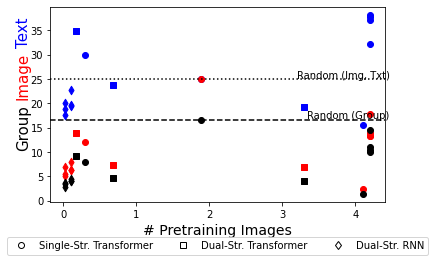
\includegraphics[width=0.49\linewidth]{figures/pretraining_images_baseline.png}}
    \subfloat{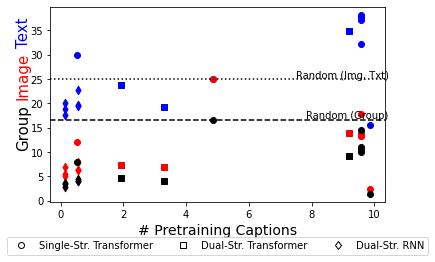
\includegraphics[width=0.49\linewidth]{figures/pretraining_captions_baseline.png}}
    \caption{Graphs of the model performance on Winoground for each model by the number of pretraining images (left) and pretraining captions (right).}
    \label{fig:pretraining_images_baseline}
\end{figure}

\subsubsection{Ours}

See \cref{tab:data-size-correlations-ours}  and \cref{fig:pretraining_images_ours}

\begin{table}[ht]
\centering
\begin{tabular}{llrr}
\toprule
Pretraining & Score & Corr. & p-value\\\midrule
               & Text    & \textbf{-0.44} & \textbf{0.04} \\
 Image              & Image   & \textbf{-0.49} & \textbf{0.02} \\
               & Group   & \textbf{-0.46} & \textbf{0.03} \\
             & Text    & \textbf{-0.44} & \textbf{0.04} \\
 Caption            & Image   & \textbf{-0.49} & \textbf{0.02} \\
             & Group   & \textbf{-0.46} & \textbf{0.03} \\
\bottomrule
\end{tabular}
\caption{Correlations between the number of pretraining images and captions and the model text, image, and group scores. Only BLIP, CLIP and FLAVA are included.}
\label{tab:data-size-correlations-ours}
\end{table}

\begin{figure}[ht]
    \centering
    \subfloat{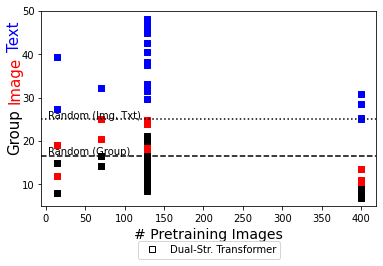
\includegraphics[width=0.49\linewidth]{figures/pretraining_images_ours.png}}
    \subfloat{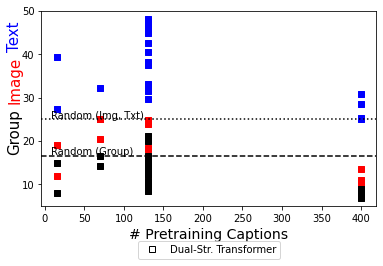
\includegraphics[width=0.49\linewidth]{figures/pretraining_captions_ours.png}}
    \caption{Graphs of the model performance on Winoground for each model by the number of pretraining images (left) and pretraining captions (right).}
    \label{fig:pretraining_images_ours}
\end{figure}